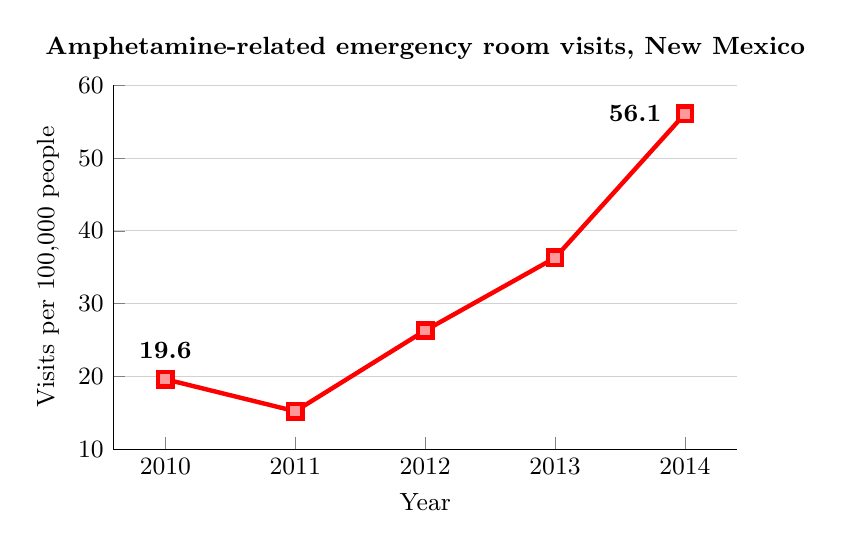
\begin{tikzpicture}
\begin{axis}[
  width=9.5cm, height=6.2cm,
  ymin=10, ymax=60, ytick={10,20,...,60},
  xmin=2009.6, xmax=2014.4, xtick={2010,...,2014},
  xticklabel style={/pgf/number format/1000 sep={}},
  ymajorgrids, grid style={gray!35},
  axis lines*=left,
  tick label style={font=\small},
  ylabel={Visits per 100,000 people}, ylabel style={font=\small},
  xlabel={Year}, xlabel style={font=\small},
  title={Amphetamine-related emergency room visits, New Mexico},
  title style={font=\small\bfseries}
]
\addplot[red, line width=1.6pt, mark=square*, mark size=2.6pt,
  mark options={fill=red!40, draw=red}]
  coordinates {(2010,19.6) (2011,15.2) (2012,26.3) (2013,36.3) (2014,56.1)};
\node[font=\small\bfseries, above=4pt] at (axis cs:2010,19.6) {19.6};
\node[font=\small\bfseries, left=5pt] at (axis cs:2014,56.1) {56.1};
\end{axis}
\end{tikzpicture}
